\documentclass[tikz]{standalone}
\begin{document}
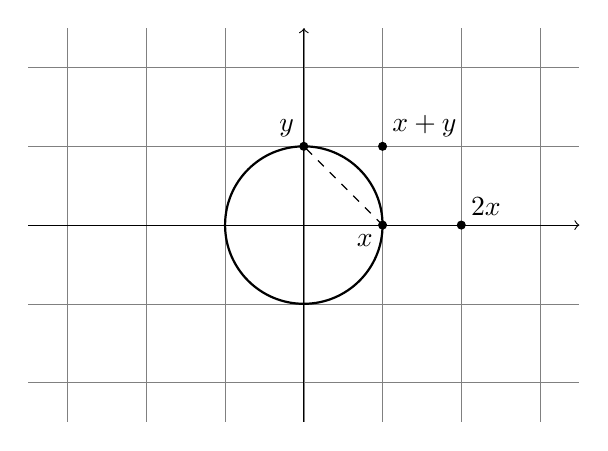
\begin{tikzpicture}
  \draw[help lines] (-3.5,-2.5) grid (3.5,2.5);
  \draw [->] (-3.5,0) -- (3.5,0);
  \draw [->] (0,-2.5) -- (0,2.5);
  \draw[thick] (0,0) circle [radius=1];
  \draw[fill] (1,0) circle [radius=0.05];
  \node [below left] at (1,0) {$x$};
  \draw[fill] (0,1) circle [radius=0.05];
  \node [above left] at (0,1) {$y$};
  \draw [dashed] (1,0) -- (0,1);
  \draw[fill] (2,0) circle [radius=0.05];
  \node[above right] at (2,0) {$2 x$};
  \draw[fill] (1,1) circle [radius=0.05];
  \node[above right] at (1,1) {$x+y$};
\end{tikzpicture}
\end{document}
